\section{Writing Sample}

We define the integral of a measurable function in three steps.

\begin{definition}[Left Coset]
Let $H$ be a subgroup of a group~$G$. A \emph{left coset} of $H$ in $G$ is a subset of $G$
of the form $xH = \{ xh : h \in H \}$.
\end{definition}

\begin{lemma}[Size of Left Coset]
Let $H$ be a finite subgroup of a group $G$. Then each left coset of $H$ in $G$ has the
same number of elements as $H$.
\end{lemma}

\begin{theorem}[Lagrange's Theorem]
Let $G$ be a finite group, and let $H$ be a subgroup of $G$. Then the order of $H$
divides the order of $G$.
\end{theorem}

\begin{proof}
Let $z \in xH \cap yH$. Then $z = xa$ for some $a \in H$ and $z = yb$ for some $b \in H$.
For any $h \in H$, $zh = x(ah)$ and $xh = z(a^{-1}h)$, so $zH = xH$. Similarly $yH = zH$,
hence $xH = yH$.
\end{proof}

\begin{figure}[!htbp]
  \centering
  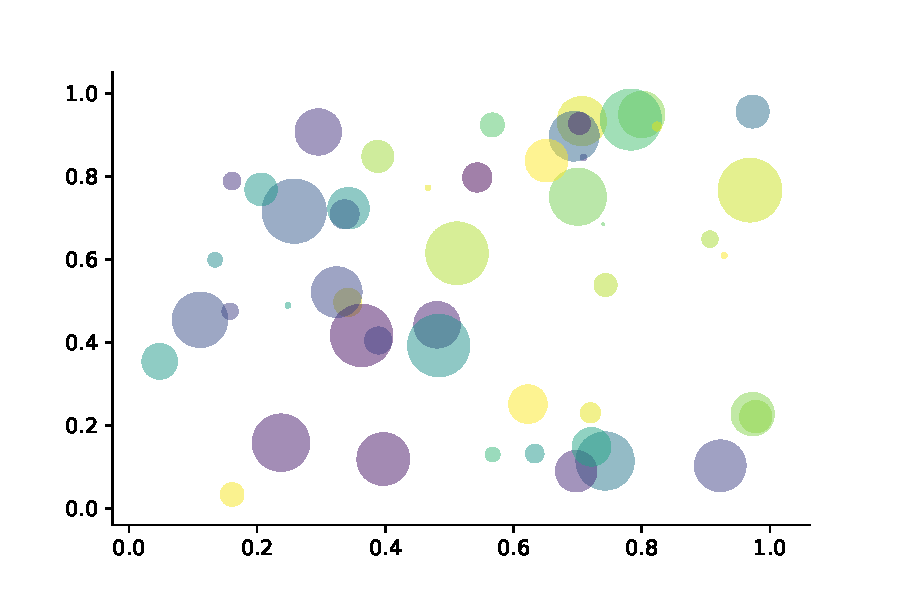
\includegraphics[width=0.6\textwidth]{images/scatter.pdf}
  \caption{Matplotlib: Scatter Plot Example\label{fig:scatter}}
\end{figure}

Regression analysis examines the relationship between variables of interest.

\begin{table}[htbp]
  \small
  \centering
  \caption{Auto MPG and Price \label{tab:reg}}
  \begin{tabular}{lcc}
    \toprule
                  & (1) & (2) \\
    \midrule
    mpg           & $-238.90^{***}$ & $-49.51$ \\
    weight        &                 & $1.75^{***}$ \\
    constant      & $11{,}253^{***}$ & $1{,}946$ \\
    obs           & 74              & 74 \\
    $R^2$         & 0.220           & 0.293 \\
    \bottomrule
    \multicolumn{3}{l}{\scriptsize *** $p<0.01$, ** $p<0.05$, * $p<0.1$}
  \end{tabular}
\end{table}
